% Overview of AnytimeSwarm (vector illustration drawn with TikZ; compile: pdflatex fig_architecture.tex)
\documentclass[tikz,border=2pt]{standalone}
\usepackage[T1]{fontenc}
\usepackage{newtxtext}
\usepackage[varvw]{newtxmath}
\usetikzlibrary{arrows.meta,calc,positioning,shapes.geometric}
\definecolor{ink}{HTML}{1F1F1F}
\definecolor{muted}{HTML}{8A877F}
\definecolor{grid}{HTML}{E4E2DB}
\definecolor{blue}{HTML}{2A78D6}
\definecolor{lblue}{HTML}{E6F0FC}
\definecolor{orange}{HTML}{E36A2E}
\definecolor{lorange}{HTML}{FFF1E2}
\definecolor{green}{HTML}{1BAF7A}
\definecolor{red}{HTML}{D83B3B}
\definecolor{lgrey}{HTML}{F4F3EF}
% quadcopter icon
\tikzset{
  drone/.pic={
    \draw[line width=0.45pt, #1] (-0.13,-0.13) -- (0.13,0.13) (-0.13,0.13) -- (0.13,-0.13);
    \foreach \x/\y in {-0.13/-0.13, 0.13/0.13, -0.13/0.13, 0.13/-0.13}
      \draw[line width=0.4pt, #1, fill=white] (\x,\y) circle (0.065);
    \fill[#1] (0,0) circle (0.045);
  },
  drone/.default=ink,
  task/.style={circle, fill=#1, inner sep=0pt, minimum size=3.2pt},
  task/.default=muted,
  panel/.style={draw=#1, line width=0.6pt, rounded corners=3pt},
  arr/.style={-{Stealth[length=4.2pt,width=3.4pt]}, line width=0.7pt, draw=ink},
  lab/.style={font=\fontsize{7.2}{8}\selectfont, text=ink},
  small/.style={font=\fontsize{6.2}{7}\selectfont, text=ink},
}
\begin{document}
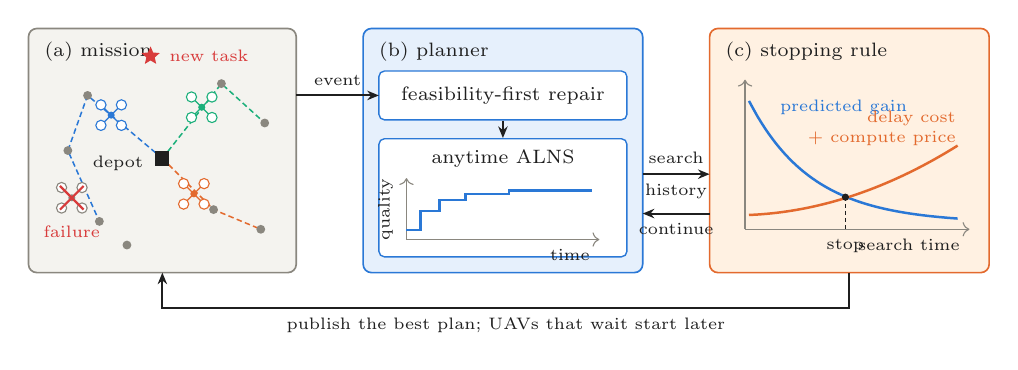
\begin{tikzpicture}[font=\fontsize{7}{8}\selectfont]
% ======================================================== (a) mission environment
\fill[lgrey, rounded corners=3pt] (0,0) rectangle (3.4,3.1);
\draw[panel=muted] (0,0) rectangle (3.4,3.1);
\node[lab, anchor=north west] at (0.08,3.05) {(a) mission};
% routes (dashed) and tasks
\coordinate (D) at (1.7,1.45);
\draw[blue, line width=0.55pt, dash pattern=on 2pt off 1.2pt] (D) -- (0.75,2.25) -- (0.5,1.55) -- (0.9,0.65);
\draw[green, line width=0.55pt, dash pattern=on 2pt off 1.2pt] (D) -- (2.45,2.4) -- (3.0,1.9);
\draw[orange, line width=0.55pt, dash pattern=on 2pt off 1.2pt] (D) -- (2.35,0.8) -- (2.95,0.55);
\foreach \p in {(0.75,2.25),(0.5,1.55),(0.9,0.65),(2.45,2.4),(3.0,1.9),(2.35,0.8),(2.95,0.55),(1.25,0.35)}
  \node[task] at \p {};
% depot
\fill[ink] ($(D)+(-0.09,-0.09)$) rectangle ($(D)+(0.09,0.09)$);
\node[small, anchor=east] at ($(D)+(-0.12,-0.06)$) {depot};
% drones
\pic at (1.05,2.0) {drone=blue};
\pic at (2.2,2.1) {drone=green};
\pic at (2.1,1.0) {drone=orange};
% event: new task (star) and failed drone (red cross)
\node[star, star points=5, star point ratio=2.2, fill=red, inner sep=0pt, minimum size=7pt] (new) at (1.55,2.75) {};
\node[small, right=1pt, text=red] at (new.east) {new task};
\pic at (0.55,0.95) {drone=muted};
\draw[red, line width=0.8pt] (0.4,0.8) -- (0.7,1.1) (0.4,1.1) -- (0.7,0.8);
\node[small, text=red, anchor=north] at (0.55,0.72) {failure};
% ======================================================== (b) planner
\begin{scope}[shift={(4.25,0)}]
\fill[lblue, rounded corners=3pt] (0,0) rectangle (3.55,3.1);
\draw[panel=blue] (0,0) rectangle (3.55,3.1);
\node[lab, anchor=north west] at (0.08,3.05) {(b) planner};
% repair box
\node[draw=blue, fill=white, rounded corners=2pt, line width=0.5pt, minimum width=3.15cm, minimum height=0.62cm,
      align=center, lab] (rep) at (1.775,2.25) {feasibility-first repair};
% anytime search box with mini profile
\node[draw=blue, fill=white, rounded corners=2pt, line width=0.5pt, minimum width=3.15cm, minimum height=1.5cm]
      (als) at (1.775,0.95) {};
\node[lab, anchor=north] at ($(als.north)+(0,-0.03)$) {anytime ALNS};
\begin{scope}[shift={(0.55,0.42)}]
  \draw[muted, line width=0.4pt, ->] (0,0) -- (2.45,0) node[small, anchor=north east] at (2.45,0) {time};
  \draw[muted, line width=0.4pt, ->] (0,0) -- (0,0.78) node[small, anchor=south east, rotate=90] at (0,0.78) {};
  \node[small, rotate=90, anchor=south] at (-0.05,0.38) {quality};
  \draw[blue, line width=0.9pt] (0,0.12) -- (0.18,0.12) -- (0.18,0.36) -- (0.42,0.36) -- (0.42,0.5) -- (0.75,0.5)
     -- (0.75,0.58) -- (1.3,0.58) -- (1.3,0.62) -- (2.35,0.62);
\end{scope}
\draw[arr] (rep.south) -- (als.north);
\end{scope}
% ======================================================== (c) stopping controller
\begin{scope}[shift={(8.65,0)}]
\fill[lorange, rounded corners=3pt] (0,0) rectangle (3.55,3.1);
\draw[panel=orange] (0,0) rectangle (3.55,3.1);
\node[lab, anchor=north west] at (0.08,3.05) {(c) stopping rule};
\begin{scope}[shift={(0.45,0.55)}]
  \draw[muted, line width=0.4pt, ->] (0,0) -- (2.85,0);
  \draw[muted, line width=0.4pt, ->] (0,0) -- (0,1.9);
  \node[small, anchor=north east] at (2.85,0) {search time};
  \draw[blue, line width=0.9pt] plot[smooth, domain=0.05:2.7] (\x, {1.65*exp(-1.25*\x)+0.08});
  \draw[orange, line width=0.9pt] plot[smooth, domain=0.05:2.7] (\x, {0.18+0.03*\x+0.11*\x*\x});
  \coordinate (X) at (1.275,0.408);
  \draw[ink, line width=0.5pt, dash pattern=on 1.5pt off 1pt] (X) -- (1.275,0);
  \fill[ink] (X) circle (1.3pt);
  \node[small, anchor=north] at (1.275,0) {stop};
  \node[small, text=blue, anchor=west] at (0.32,1.55) {predicted gain};
  \node[small, text=orange, anchor=east, align=right] at (2.8,1.28) {delay cost\\ + compute price};
\end{scope}
\end{scope}
% ======================================================== flow arrows
\draw[arr] (3.4,2.25) -- node[small, above] {event} (4.25+0.2,2.25);
\draw[arr] (7.8,1.25) -- node[small, above] {search} node[small, below] {history} (8.65,1.25);
\draw[arr] (8.65,0.75) -- node[small, below] {continue} (7.8,0.75);
\draw[arr] (10.425,0) -- (10.425,-0.45) -- node[small, below] {publish the best plan; UAVs that wait start later} (1.7,-0.45) -- (1.7,0);
\end{tikzpicture}
\end{document}
